\documentclass[12pt, a4paper]{article}
\usepackage[a4paper, bindingoffset=0.2in, %
left=0.5in,right=0.5in,top=0.5in,bottom=0.5in,%
footskip=.25in]{geometry}
\usepackage{graphicx}
\usepackage{amssymb}
\usepackage{amsmath}
\usepackage{hyperref}
\usepackage{physics}

\title{Report of HW9}
\author{Muhammad Jamshidi \\ 98100718}
\date{}


\begin{document}
	\maketitle
	\section{First Order Differential Equation}
	\textbf{Code: \texttt{q1\textbackslash q1.py}}
	\newline
	We want to solve the first order differential equation below; Which governs the evolution of the charge of the capacitor in an RC circuit.
	\begin{equation}
		\label{eq:RC_equation}
		R \dv{Q}{t} + \frac{Q}{C} = V.
	\end{equation}
	First, we try to make a dimensionless equation; It is easy to do by using the variable change below.
	\begin{equation} \label{eq: variable_change}
		\begin{aligned}
					&x \equiv \frac{Q}{CV} - 1, \quad \tau \equiv \frac{t}{R C}\\
					\Rightarrow  &\dv{x}{\tau} + x = 0.
		\end{aligned}
	\end{equation}
	The analytical solution to this equation is
	\begin{equation}
		x = x_0 \exp(- \tau) \Rightarrow Q = C V (1 - e^{- \frac{t}{R C}}).
	\end{equation}
	This result is obtained simply by integrating the equation $\frac{\dd{x}}{x} = -\dd{\tau}$.
	I did the simulation for $t = 21 ms$ or equally $\tau = 7$, $h = 10^{-4}$, 
	$R = 3\times10^3 \Omega$, $V = 10 V$, $C = 10^{-6} F$ and zero initial charge. The result of simulation and comparison with analytical solution is given in the figure (\ref{fig:q1_euler}).
		\begin{figure}[h]
			\centering
			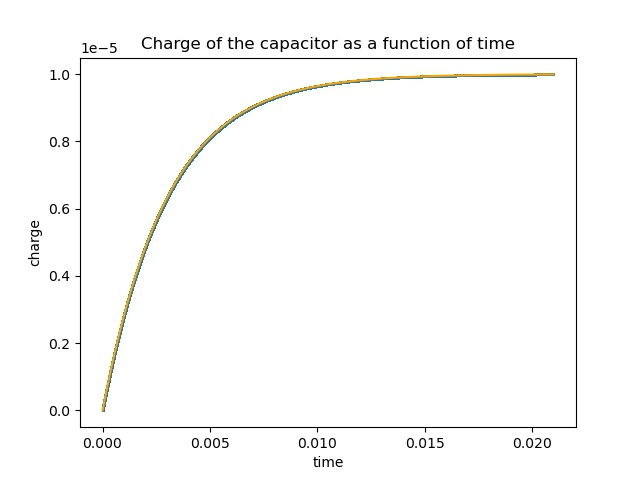
\includegraphics[width=0.8\linewidth]{../q1/q1_Euler_result_h=1e-05_tau_stop=7.0.jpg}
			\caption{Analytical and numerical solution for the charging capacitor equation. The time step for the numerical solution here is $3\times10^{-8} s$}
			\label{fig:q1_euler}
		\end{figure}
	The simulation result is in good matching with the analytical procedure. Finally, Euler's method relative error calculated and plotted for each varying h value in the figure (\ref{fig:q1_euler_error}). The slope of the best fitted line is approximately 0.993 and this
	result is in good matching with theoretical procedure.
		\begin{figure}[h]
			\centering
			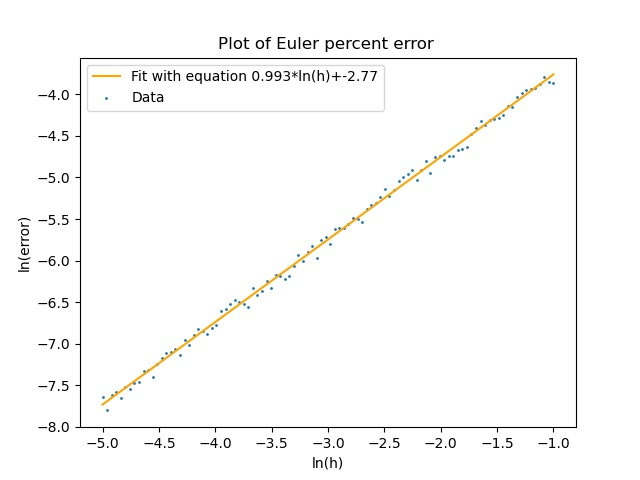
\includegraphics[width=0.8\linewidth]{../q1/q1_Euler_error_1e-05_0.1_100_0.021.jpg}
			\caption{Analytical and numerical solution for the charging capacitor equation. The time step for the numerical solution here is $3\times10^{-8} s$}
			\label{fig:q1_euler_error}
		\end{figure}
	\section{Second Order Diffrential Equation and Comparison of Algorithms}
	\textbf{Code: \texttt{q2\textbackslash q2.py}}
	\newline
	The simulation in this problem is done by using $h = 0.01$ as time step and $x_0 = 1, v_0 = 0$ as initial conditions.
	For some methods like Verlat's method I had to define extended initial conditions due to the instinct of the algorithms. 
	The result of each method is plotted in the figure (\ref{fig:q2_results_of_methods}).
		\begin{figure}[h]
			\centering
			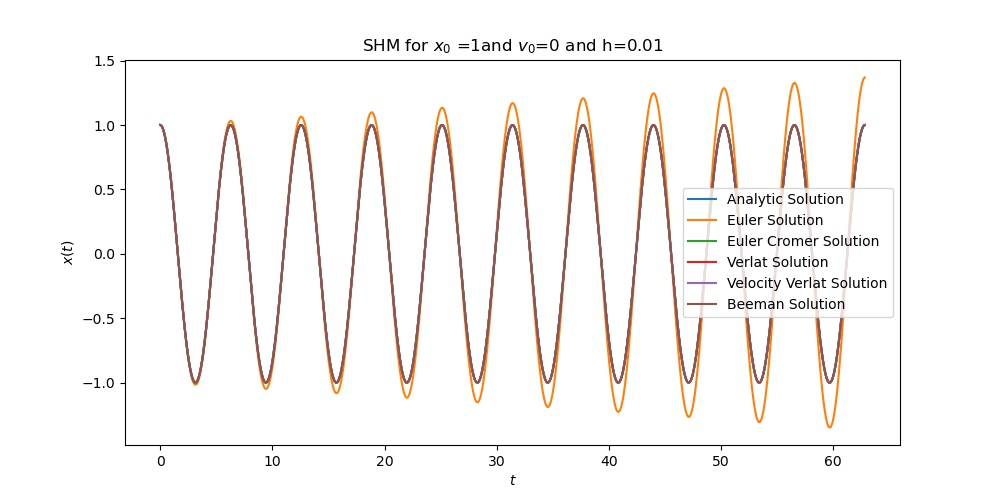
\includegraphics[width=0.8\linewidth]{../q2/q2_x_t_0_62.83185307179586_0.01_x0=1_v0=0.jpg}
			\caption{Plot of the simulation results using different methods from 0 to 20$\pi$ with time step equal to 0.01.}
			\label{fig:q2_results_of_methods}
		\end{figure}
	It is obvious from the figure(\ref{fig:q2_results_of_methods}) that the Euler-Cromer, Verlat, velocity Verlat and Beeman methods are stable algorithms for this simulation; in other words,
	Euler method doesn't keep energy of the system constant.\\
	Finally, I made plot of the phase space for each method. The plots are available in the 
	figures \ref{fig:q2_phase_space_anaytic} to \ref{fig:q2_phase_space_Beeman}. As it is 
	obvious, the plots are circles for all methods except Euler method; which is a sign of 
	changing the total mechanical energy of the system.
		\begin{figure}[h]
			\centering
			\begin{minipage}[b]{0.4\textwidth}
				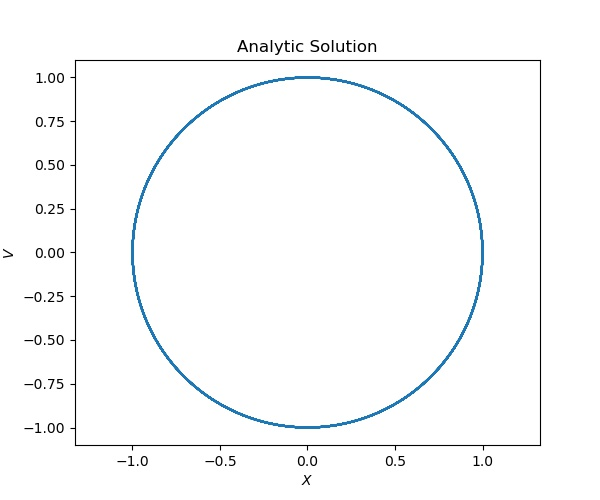
\includegraphics[width=\textwidth]{../q2/q2_v_x_Analytic Solution_0_62.83185307179586_0.01_x0=1_v0=0.jpg}
				\caption{Phase space of the system due to the anaytical method. Time step
				is 0.01, initial velocity is 0 and initial position is 1.}
				\label{fig:q2_phase_space_anaytic}
			\end{minipage}
			\hfill
			\begin{minipage}[b]{0.4\textwidth}
				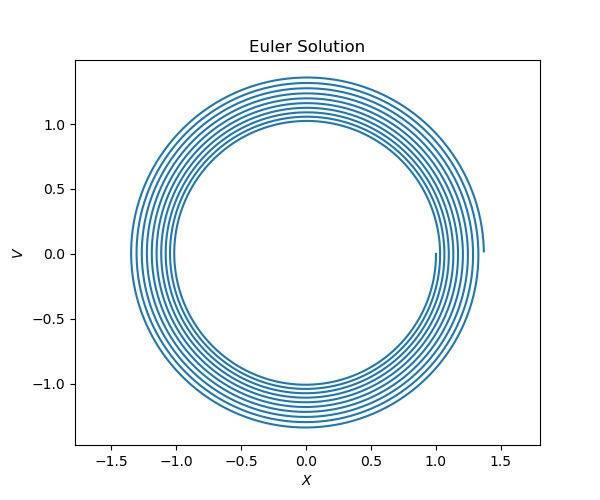
\includegraphics[width=\textwidth]{../q2/q2_v_x_Euler Solution_0_62.83185307179586_0.01_x0=1_v0=0.jpg}
				\caption{Phase space of the system due to the Euler method. Time step
				is 0.01, initial velocity is 0 and initial position is 1.}
				\label{fig:q2_phase_space_Euler}
			\end{minipage}
			\begin{minipage}[b]{0.4\textwidth}
				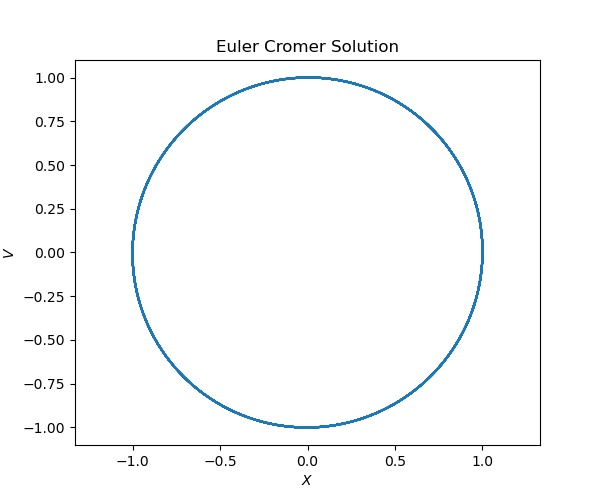
\includegraphics[width=\textwidth]{../q2/q2_v_x_Euler Cromer Solution_0_62.83185307179586_0.01_x0=1_v0=0.jpg}
				\caption{Phase space of the system due to the Euler-Cromer method. Time step
				is 0.01, initial velocity is 0 and initial position is 1.}
				\label{fig:q2_phase_space_Euler_Cromer}
			\end{minipage}
			\hfill
			\begin{minipage}[b]{0.4\textwidth}
			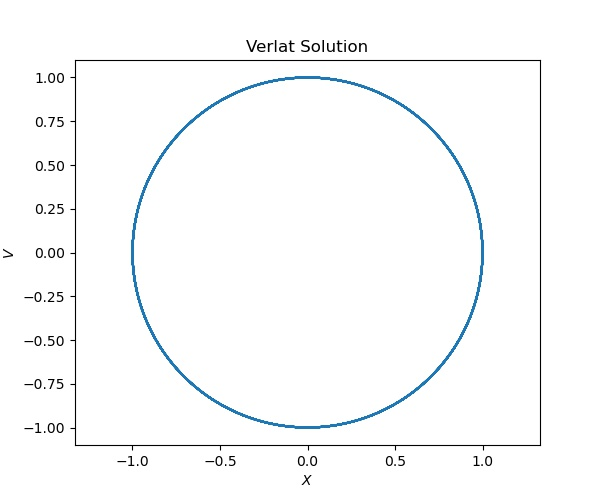
\includegraphics[width=\textwidth]{../q2/q2_v_x_Verlat Solution_0_62.83185307179586_0.01_x0=1_v0=0.jpg}
			\caption{Phase space of the system due to the Verlat method. Time step
			is 0.01, initial velocity is 0 and initial position is 1.}
			\label{fig:q2_phase_space_Verlat}
			\end{minipage}
			\hfill
			\begin{minipage}[b]{0.4\textwidth}
			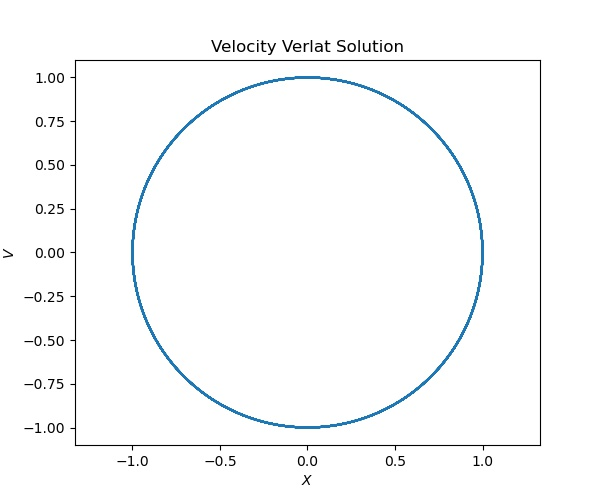
\includegraphics[width=\textwidth]{../q2/q2_v_x_Velocity Verlat Solution_0_62.83185307179586_0.01_x0=1_v0=0.jpg}
			\caption{Phase space of the system due to the velocity Verlat method. Time step
			is 0.01, initial velocity is 0 and initial position is 1.}
			\label{fig:q2_phase_space_velocity_Verlat}
			\end{minipage}
			\hfill
			\begin{minipage}[b]{0.4\textwidth}
			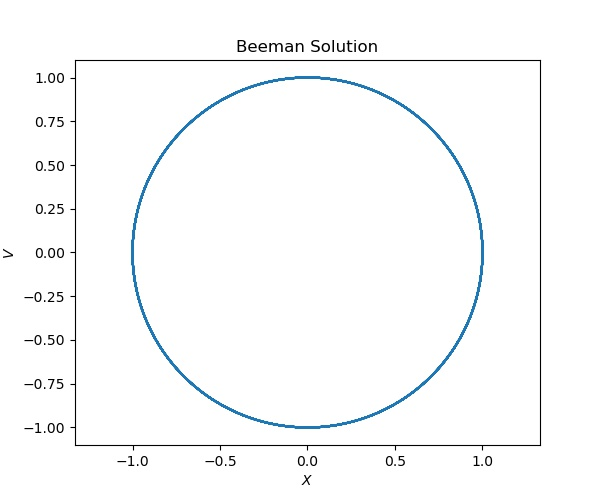
\includegraphics[width=\textwidth]{../q2/q2_v_x_Beeman Solution_0_62.83185307179586_0.01_x0=1_v0=0.jpg}
			\caption{Phase space of the system due to the Beeman method. Time step
			is 0.01, initial velocity is 0 and initial position is 1.}
			\label{fig:q2_phase_space_Beeman}
			\end{minipage}
		\end{figure}
	\section{Instability in Algorithms}
	\textbf{Code: \texttt{q3\textbackslash q3.py}}
	\newline
	In this problem I did a simulation for the equaiton (\ref{eq:RC_equation}) using the given 
	algorithm below. \\
		\begin{equation}
			y_{n+1} = y_{n-1} + 2h\dot{y}_{n}
			\label{eq:q3}
		\end{equation}
	
    The result is plotted in the figure (\ref{fig:q3}).
	Doing this simulation I used the variable change in the problem 1.
		\begin{figure}[h]
			\centering
			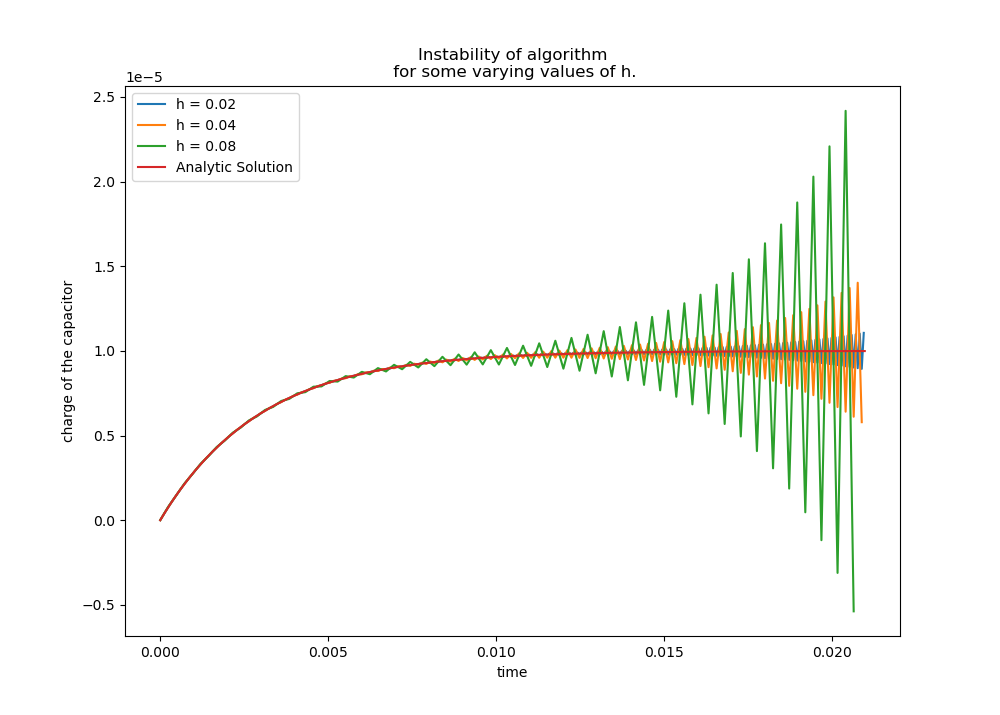
\includegraphics[width=0.8\linewidth]{../q3/q3.png}
			\caption{Simulation result using the given algorithm in equaiton (\ref{eq:q3}) and comparison with
			analytical solution.}
			\label{fig:q3}
		\end{figure}
	According to the figure (\ref{fig:q3}), the algorithm in equation (\ref{eq:q3})
	is more instable for bigger value of \textit{h}; where \textit{h} is time step in changed
	variable units (eq.\ref{eq: variable_change}).
	\section{Chaos}
	\textbf{Code: \texttt{q4\textbackslash q4.py}}
	\newline
	For calculating the periodic values of \textit{x} for each \textit{r}, I considered some random
	initial values for \textit{x} in the interval
	$[0, 1)$.
	Then I did run the recursive equation (\ref{eq:q4_recursive_equation}) on each initial \textit{x} for some given \texttt{$n_{max}$} as the number of iterations. The resulted
	plot is given in the figure (\ref{fig:q4_landscape}).
		\begin{equation}
			x_{n+1} = 4rx_{n}(1-x_{n})
			\label{eq:q4_recursive_equation}
		\end{equation}
		\begin{figure}[h]
			\centering
			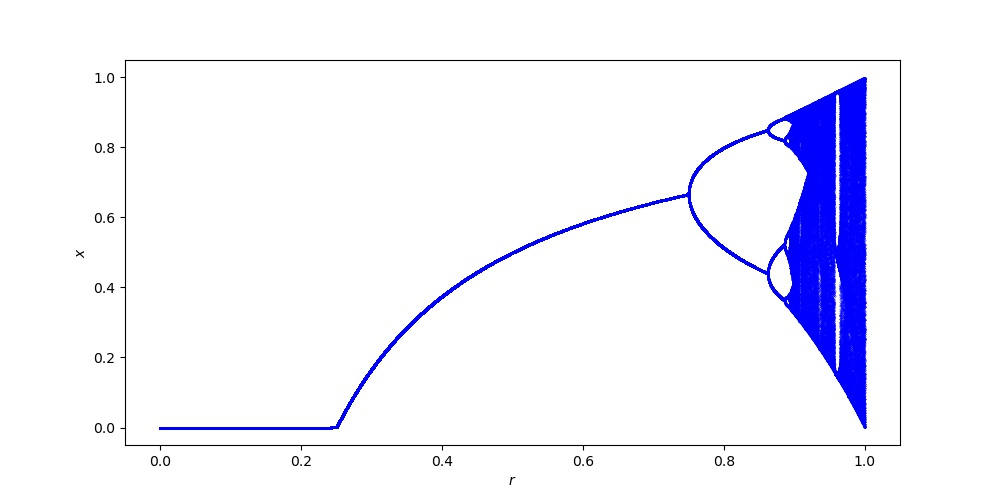
\includegraphics[width=0.8\linewidth]{../q4/q4_0_1_10000_100_1000.jpg}
			\caption{Bifurcation plot for $\Delta r=10^{-4}$ and 100 \textit{x} for each 
				\textit{r} and number of iterations is $10^3$.}
			\label{fig:q4_landscape}
		\end{figure}
	Then I did more exact simulation for calculating $r_n$ values. The results are given
	in the figures (\ref{fig:q4_r0}) to (\ref{fig:q4_r_infinity}).
	\begin{figure}[h]
		\centering
		\begin{minipage}[b]{0.4\textwidth}
		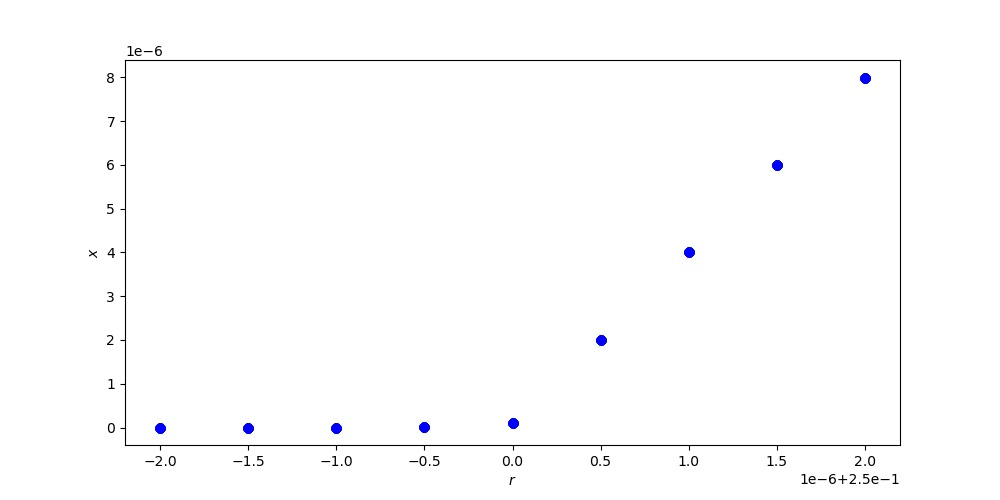
\includegraphics[width=\textwidth]{../q4/q4_0.249998_0.250002_9_100_10000000.jpg}
		\caption{Bifurcation plot about $r_0$ for $\Delta r=10^{-6}$ and 100 \textit{x} for each 
			\textit{r} and number of iterations is $10^7$.}
		\label{fig:q4_r0}
		\end{minipage}
		\hfill
		\begin{minipage}[b]{0.4\textwidth}
		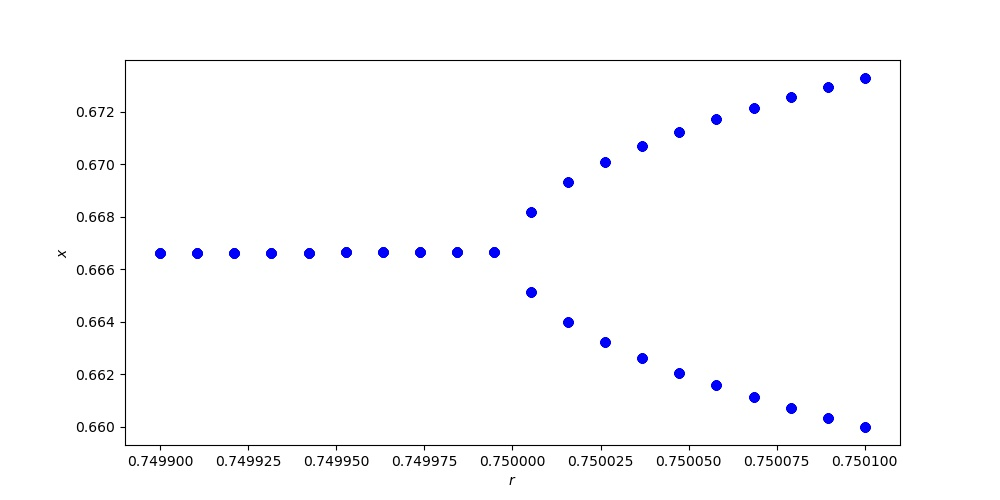
\includegraphics[width=\textwidth]{../q4/q4_0.7499_0.7501_20_100_1000000.jpg}
		\caption{Bifurcation plot about $r_1$ for $\Delta r=10^{-5}$ and 100 \textit{x} for each 
			\textit{r} and number of iterations is $10^6$.}
		\label{fig:q4_r1}
		\end{minipage}
		\hfill
		\begin{minipage}[b]{0.4\textwidth}
		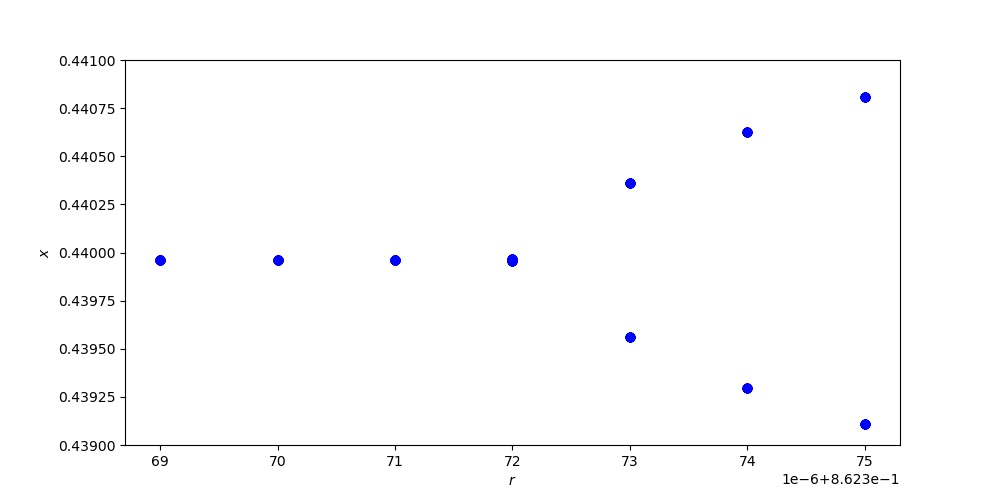
\includegraphics[width=\textwidth]{../q4/q4_0.8623689999999999_0.862375_7_100_1000000.jpg}
		\caption{Bifurcation plot about $r_2$ for $\Delta r=10^{-6}$ and 100 \textit{x} for each 
				\textit{r} and number of iterations is $10^6$.}
		\label{fig:q4_r2}
		\end{minipage}
		\hfill
		\begin{minipage}[b]{0.4\textwidth}
		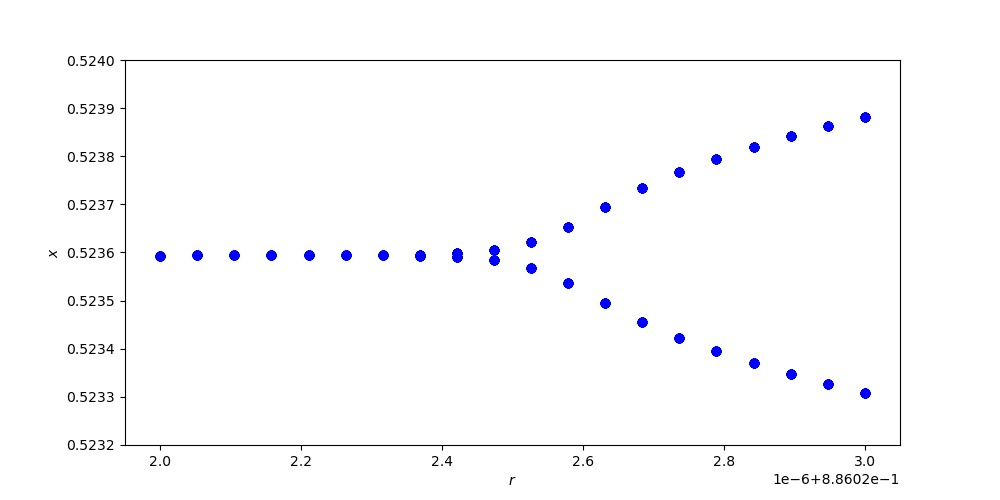
\includegraphics[width=\textwidth]{../q4/q4_0.886022_0.886023_20_100_1000000.jpg}
		\caption{Bifurcation plot about $r_3$ for $\Delta r=5\times10^{-8}$ and 100 \textit{x} for each 
		\textit{r} and number of iterations is $10^6$.}
		\label{fig:q4_r3}
		\end{minipage}
		\hfill
		\begin{minipage}[b]{0.4\textwidth}
		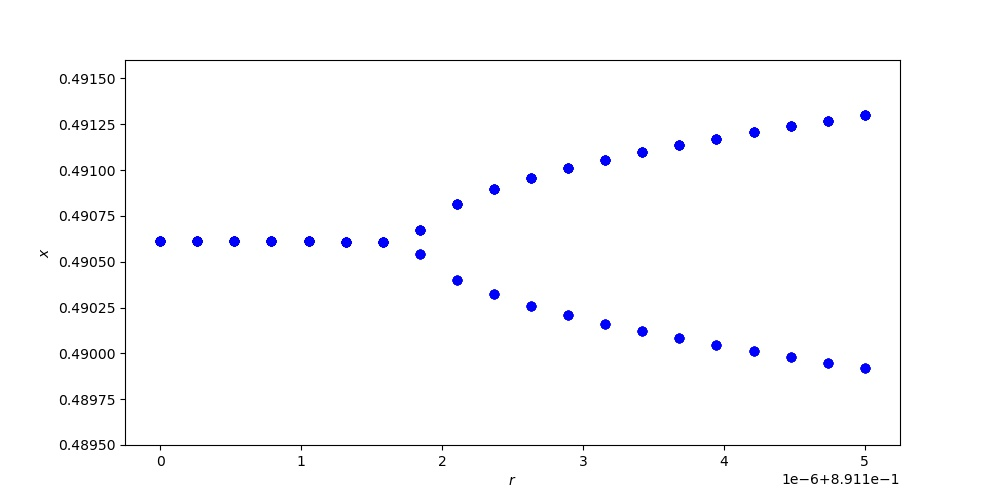
\includegraphics[width=\textwidth]{../q4/q4_0.8911_0.891105_20_100_1000000.jpg}
		\caption{Bifurcation plot about $r_4$ for $\Delta r=2.5\times10^{-7}$ and 100 \textit{x} for each 
		\textit{r} and number of iterations is $10^6$.}
		\label{fig:q4_r4}
		\end{minipage}
		\hfill
		\begin{minipage}[b]{0.4\textwidth}
		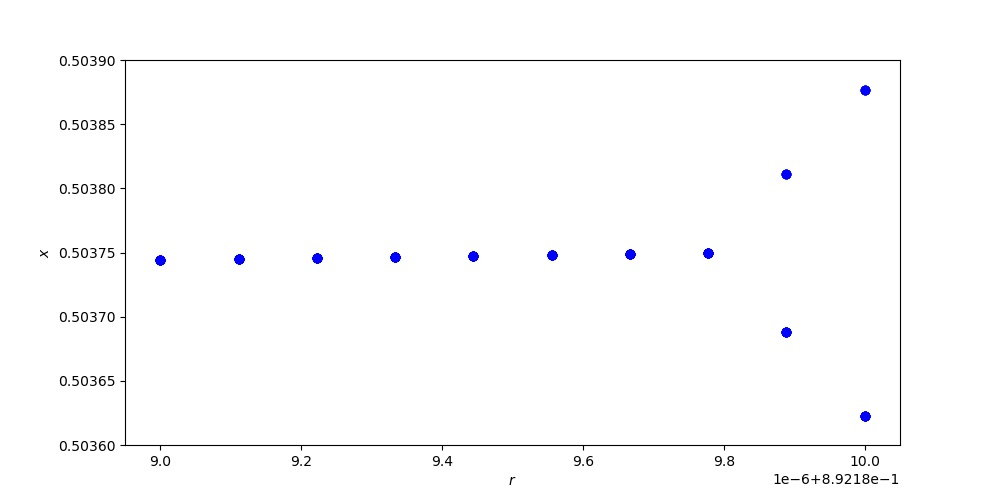
\includegraphics[width=\textwidth]{../q4/q4_0.892189_0.89219_10_100_1000000.jpg}
		\caption{Bifurcation plot about $r_5$ for $\Delta r=10^{-6}$ and 100 \textit{x} for each 
		\textit{r} and number of iterations is $10^6$.}
		\label{fig:q4_r5}
		\end{minipage}
		\hfill
		\begin{minipage}[b]{0.4\textwidth}
		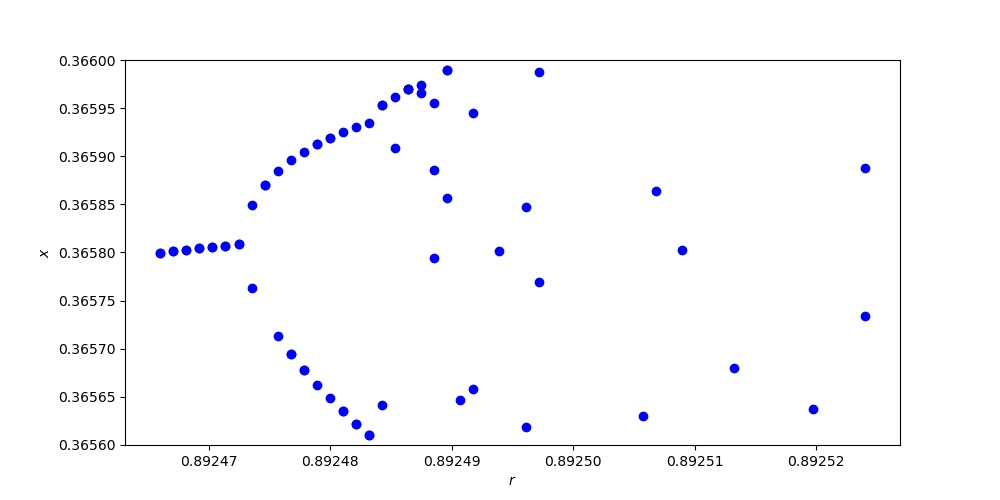
\includegraphics[width=\textwidth]{../q4/q4_0.8924660000000001_0.892524_55_100_1000000.jpg}
		\caption{Bifurcation plot about $r_{\infty}$ for $\Delta r=10^{-6}$ and 100 \textit{x} for each 
		\textit{r} and number of iterations is $10^6$.}
		\label{fig:q4_r_infinity}
		\end{minipage}
		\hfill
	\end{figure}
	According to the figures (\ref{fig:q4_r0}) to (\ref{fig:q4_r_infinity}), I concluded the results given in (\ref{eq:q4_r_n}).
	\begin{equation}
		\begin{cases}
			r_0 = 0.250000 \pm 10^{-6} \\
			r_1 = 0.749999 \pm 10^{-6} \\
			r_2 = 0.862372 \pm 10^{-6} \\
			r_3 = 0.886020 \pm 10^{-6} \\
			r_4 = 0.891101 \pm 10^{-6} \\
			r_5 = 0.892189 \pm 10^{-6} \\
			r_\infty = 0.892487 \pm 10^{-6}
		\label{eq:q4_r_n}
		\end{cases}
	\end{equation}
	Using the values in (\ref{eq:q4_r_n}), I calculated the $\delta$ parameter using the 
	formula $\delta \approx \frac{r_4 - r_3}{r_5 - r_4}$. I found $\delta \approx 4.668.$
	Finally for calculating the value of $\alpha$, I had to calculate the values of \textit{r}s,
	say $r_3$ and $r_4$, more exactly. So I did the simulation more exactly about points $r_3$
	and $r_4$. Resulted plots are given in the figures (\ref{fig:q4_r3_prime}) and (\ref{fig:q4_r4_prime}). Resulted more exact values for $r_3$ and $r_4$ are given in (\ref{eq:q4_r_3_4_prime}).
	\begin{figure}
		\centering
		\begin{minipage}[b]{0.4\textwidth}
			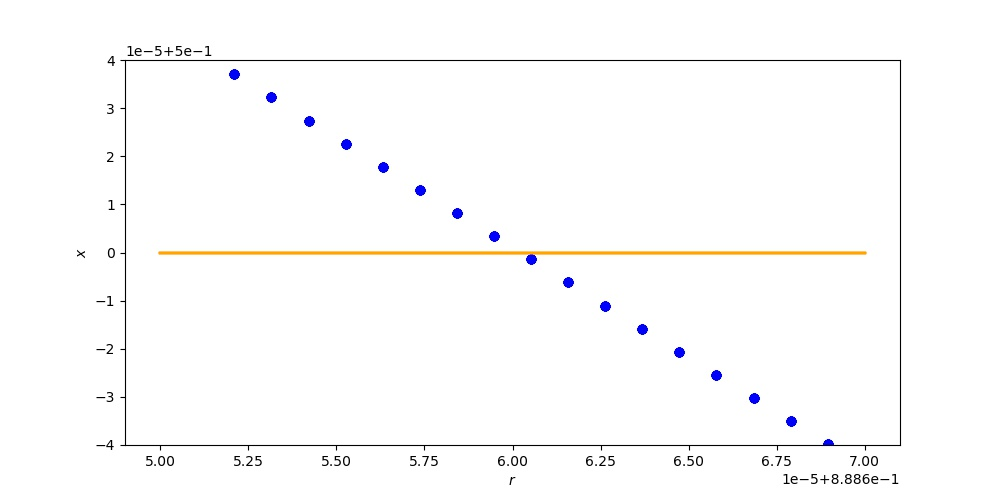
\includegraphics[width=\textwidth]{../q4/q4_0.8886499999999999_0.88867_20_100_100000.jpg}
			\caption{Bifurcation plot about $r_3$ for $\Delta r=10^{-6}$ and 100 \textit{x} for each 
			\textit{r} and number of iterations is $10^5$.}
			\label{fig:q4_r3_prime}
		\end{minipage}
		\hfill
		\begin{minipage}[b]{0.4\textwidth}
			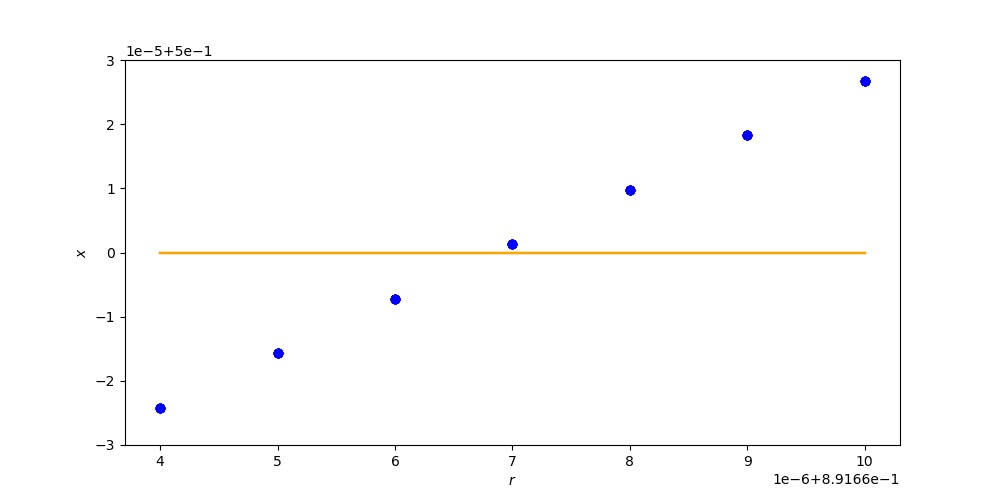
\includegraphics[width=\textwidth]{../q4/q4_0.891664_0.89167_7_100_1000000.jpg}
			\caption{Bifurcation plot about $r_4$ for $\Delta r=10^{-6}$ and 100 \textit{x} for each 
			\textit{r} and number of iterations is $10^5$.}
			\label{fig:q4_r4_prime}
		\end{minipage}
	\end{figure}
	\begin{equation}
		\begin{cases}
			r_3 = 0.888660 \pm 10^{-6} \\
			r_4 = 0.891667 \pm 10^{-6} \\
		\end{cases}
		\label{eq:q4_r_3_4_prime}
	\end{equation}
	Finally I calculated the length of the mouth of the plot, near the $r_3$ and $r_4$ and found the parameter $\alpha$ as given in the equation (\ref{eq:q4_alpha}).
	\begin{equation}
		\alpha \approx \frac{0.04597434}{-0.01833120} \Longrightarrow
		\alpha \approx -2.507
		\label{eq:q4_alpha}
	\end{equation}









\end{document}